\chapter{分布式大数据内存计算系统Spark系统实现机制概述}\label{chap:basic}
\section{Spark系统实现概述概述}
Spark是一种基于内存的分布式计算框架。Spark框架分为四层:用户层、作业管理执行层、资源任务调度层、物理执行层。在用户层,用户需要使用框架api编写应用代码,准备输入数据,配置应用参数。用户将这些信息提交给作业管理执行层后,框架会将用户应用转化为具体的作业执行计划,分为逻辑处理计划(数据单元和数据处理依赖关系)和物理执行计划(具体执行计划和阶段)。生成了具体的执行计划之后,框架的资源任务调度层会向集群资源管理器申请资源,资源申请成功后,框架把具体任务和资源绑定,并发送作业执行计划给物理执行层。物理执行层收到作业执行计划之后,会根据作业的配置信息下载应用代码,运行任务并将执行结果反馈给框架。下面会对Spark框架的四层进行进一步的介绍。

\begin{enumerate}
    \item 用户层:用户层提供了丰富的应用接口。包括面向结构化数据的查询接口Spark SQL,面向图计算的GraphX、面向机器学习的Spark MLlib,面向实时流计算的Spark Stream。用户使用提供的接口可以实现丰富的应用程序。
    \item 作业管理执行层:框架收到用户提交的应用程序后,就将其解析成Spark可以识别的逻辑执行计划。比如对于Spark SQL作业,会通过SQL语言的解释器将SQL语句解释为Spark可识别的作业执行计划,一般是以DAG(Directed Acycilc Graph)有向无环图结构组成的作业执行计划。Spark框架会遍历DAG,如果遇到需要Shuffle的边就会对当前边进行切割。遍历完毕之后整个DAG被切割成多个子图,每个子图都会更具拓扑顺序从前到后逐渐调度执行。
    \item 资源任务调度层:Spark框架一般是主从(Master-Slave)架构。主节点负责接受用户的应用,解析作业,管理执行作业,并在出错场景下做容错管理。从节点主要负责接受主节点的任务执行计划,具体执行作业并将结果汇总给主节点。
    \item 物理执行层:物理执行层会执行真正的任务。物理执行层下载或者接受得到用户代码,申请内存开始执行,将执行结果存入特定文件或者通过网络发送给下游节点。任务执行过程中需要内存,输出临时数据也需要在内存中缓存。执行结束之后框架会将执行结果发送给框架。
\end{enumerate}

\section{Spark系统整体架构}
Spark框架系统架构采用了Master-Worker结构。Master节点负责管调度理应用,Worker负责具体执行任务。Master节点会管理监控所有的Worker节点,并且调度执行应用作业,将任务调度给Worker节点,监控收集Worker节点上任务的执行状况。Worker节点会定时和Master节点进行心跳交互。收到Master节点发送的任务后后在本地执行任务,并监控任务状态,将任务执行状况上报给Master节点。具体有一下几个概念需要解释。

Spark Application,Spark应用指的是一个可运行的Spark程序。程序中包含main函数,一般流程是从数据源读取输入数据,进行一系列的处理,计算的到结果后保存到磁盘中。应用程序包含了一些配置参数,例如需要使用的CPU个数,Executor内存大小等。用户可以直接使用Spark提供的接口实现程序,也可以使用Spark SQL编写程序,Spark SQL框架会将SQL查询语言转化成一个Spark应用。

Spark Driver,Spark驱动程序是指运行Spark应用main函数的进程,它会创建Spark Context。一般是指Master节点运行的Spark应用进程,Driver进程独立于Master进程。Driver进程会通过DAGScheduler、TaskScheduler、SchedulerBackEnd等模块调度调度应用中的具体任务。

Executor,Spark执行器是Spark集群的一个资源单位。Spark Driver会向Yarn、K8s等资源调度器申请资源,资源分配成功之后会启动一个Executor进程。之后Spark Driver通过DAGScheduler和TaskScheduler调度执行作业,并通过SchedulerBackend将具体任务发送给Executor。Executor收到任务请求后会在本地JVM虚拟机创建进程执行任务。

Task,Spark计算任务。Driver程序启动后会将Spark应用切分成多个计算任务,然后调度给Executor执行。Task是最小的计算任务,Executor会给每个Task分配一个JVM进程,执行具体的计算任务,如Map算子、Filter算子、Reduce算子等。Executor一般会占用多个CPU,Task一般使用一个CPU,所以Executor中可以执行多个Task,所有Task共享Executor的内存。

这几个概念中Driver需要进一步解释。Driver包含SparkContext对象,SparkContext会将应用程序转化成一个DAG图,之后遍历DAG图,如果遇到一个action操作,也就是需要具体计算结果的操作,SparkContext就会给DAGScheduler提交一个Job。DAGScheduler收到Job请求之后会从后向前遍历作业,如果遇到边是窄依赖,就会将当前节点加入当前Stage,如果遇到的边是宽依赖,也就是需要Shuffle的边,DAGScheduler就会创建一个新的Stage,并将该节点加入新的Stage之中。遍历结束之后会得到许多个Stage,DAGScheduler会将Stage打包成TaskSet后发送给TaskScheduler执行。TaskScheduler后根据调度策略选择合适的Executor调度执行计算任务。执行结束之后Executor会讲结果汇总发送给Driver。


\section{Spark内存管理模块分析}

Spark是一种基于内存的分布式计算框架,在计算的过程中通过将数据缓存在内存中加速计算过程。所以内存管理模块是Spark系统的核心模块。Spark内存管理机制在JVM虚拟内存管理的基础上对Executor模块拥有的内存进行了进一步的分配管理。也支持在Executor外的系统内存中直接开辟内存空间用于存储计算过程中产生的大量数据。通过使用对外内存,可以减少内存空间不足导致的垃圾回收以及内存不足错误。

Spark框架执行过程中内存管理模块会申请JVM内存,申请的大小由配置参数决定。内存管理模块会将内存分为四个部分。Storage Memory,Execution Memory,User Memory,Reserved Memory。四部分内存有不同的用途。

\begin{enumerate}
    \item Storage Memory 用于缓存中间数据。比如对于一份数据data1,在之后计算过程中需要重复使用。就可以调用data1.cache接口将数据缓存在Storage Memory区域。在之后计算过程中框架就可以直接从Storage Memory区域读取数据。具体来说,调用cache接口并不会立刻将数据写入缓存之中,而只是设置了STORAGE\_LEVEL这个标记为MEMORY\_ONLY。后续在框架执行的过程中,当data1被计算得到时,框架会检查STORAGE\_LEVEL这个标记,发现为MEMORY\_LEVEL后会通过memory maneger将其存入Storage Memory之中。这个过程并不会造成内存拷贝复制。memory manager只是将指向数据的引用从Execution Memory移到Storage Memory之中,并更新两个内存区域内存总量。
    
    \item Execution Memory 用于框架计算过程。在计算过程中比如对于Shuffle操作,需要在内存中缓存一部分数据,再一次性写入文件系统之中,从而避免频繁磁盘IO导致的延迟。在计算的过程中数据也都存放在Executor Memory之中。比如上面所说的data1,在计算过程中一直使用Execution Memory。在计算结束之后根据STORAGE\_LEVEL,如果为MEMORY\_ONLY就会移到Storage Memory之中。
    
    \item User Memory 为应用程序使用的内存空间。应用程序创建的各种和Spark框架无关的对象都会存在User Memory之中。
    
    \item Reserved Memory 的目的是避免发生OOM(Out of Memory)错误。OOM问题的根本原因是框架的内存管理和底层JVM的内存管理是完全隔离的。框架只是简单的记录内存的使用量,但是记录的内存使用量和实际的内存使用量并不是一一对应的。首先User Memory的内存是框架无法准确感知的。其次Storage Memory区域的内存也是不准确的,比如Storage Memory区域缓存有一份数据data1。之后应用程序调用data1.uncache接口将data1数据从内存中清除。框架所做的工作是在缓存管理模块中将data1的引用释放,并且将data1的内存总量加到Storage Memory的空闲内存之中,表示这些内存空间空闲。但是此时data1实际占用的JVM内存并没有被释放,实际内存的释放完全依赖于JVM虚拟机的垃圾回收机制,如果此时框架有新的内存申请请求,就有很大可能让框架实际使用内存超过向JVM申请的资源,导致OOM错误。所以需要保留一段空闲内存,避免这种OOM的出现。但是这种方法也有一些缺点,首先它并不能完全消除OOM错误,只要多申请的内存超过Reserved Memory的大小,还是会导致出错。另一方面Reserved Memory所占用的内存资源完全被浪费了,造成内存资源利用率下降。
\end{enumerate}

目前内存管理模块有两种模式,默认模式和Legacy模式。默认模式Storage Memory和Execution Memory是共享内存空间的。Legacy模式下Storage Memory和Execution Memory是隔离的,通过配置文件可以配置两者的大小。

\subsection{弹性分布式数据集RDD}

弹性分布式数据集(Resilient Distributed Datasets)是Spark框架的核型概念。RDD是指一种可并行可操作的只读数据集合。RDD利用了Scala语言的特性,Scala将数据分为可变数据variable和不可变数据value。RDD中的数据被设置成不可变数据,所以在创建之后就不能再改变了,因为是不可变数据,所以很适合并行处理。RDD数据有丰富的操作,操作也分为两类,transform和action。transform操作是将一个RDD转化为另一个RDD。因为对于用户来说RDD无法直接展示,所以框架也不会立即计算。action操作是计算出一个具体的结果,比如求和,求平均数等操作。因为需要计算具体的结果,所以框架只有遇到action操作才会具体计算。RDD数据之间的操作相当于作业DAG图中的边。RDD相当于DAG图中的点。Spark框架通过DAG图的拓扑来解决容错的问题。比如data1是由data2和data3计算得到的。在DAG图中就有data1指向data2和data3的两条边。在计算data1的过程中框架会沿着这两天边检查data2和data3的状态,如果data2和data3保存在内存之中,框架会直接进行计算,如果保存在磁盘之中,框架会从磁盘中将数据加载到内存之中进行计算。如果数据完全丢失了,框架就会重新计算RDD数据。

RDD之间的关系还可以进一步分类。如果转化操作的逻辑可以转化为窄依赖和宽依赖两种。窄依赖是指父RDD的每个分区只被一个子RDD的分区使用,这种依赖关系下,父子RDD之间数据交换无需进行shuffle操作,父RDD只需将数据发送给子RDD即可。宽依赖是指父RDD的分区数据会被多个子RDD的分区使用,也就是说父RDD输出的数据会被多个子RDD使用,这就需要在父子之间进行Shuffle交换数据,宽窄依赖主要用于作业调度执行。框架在执行过程中遇到一个action操作就会提交一个job,在job调度执行期间,DAGScheduler会把所有宽依赖所在的边切分,将整个DAG计算图切分成多个子图,每个子图称为一个stage,DAGScheduler将stage发送给TaskScheduler调度执行每一个任务。

\subsection{作业执行调度模块}

调度模块主要有这几部分:ResourceManager,DAGScheduler,TaskScheduler,SchedulerBackend。其中ResourceManger用于向资源调度器,如Yarn,Mesos,Kubernetes申请资源。资源申请成功之后会启动一个Executor进程。Executor进程启动之后会向Driver进程反向注册,注册成功之后也会持续发送心跳包,同时等待Driver下发任务。收到任务后Executor会执行并上报任务执行状态。这就是资源调度的基本过程。

在任务调度方面,用户的应用程序会根据RDD之间的转化关系转化成一个DAG图,之后框架会将DAG分成多个job,每个job会分成多个stage,stage中的任务会组成taskSet发送给Executor执行,这里详细解释一下这几个概念。

\begin{enumerate}
    \item Application, 用户编写的Spark应用程序,应用提交给Spark框架后框架会将应用转换成框架可以识别的DAG图,并对DAG图进行遍历,遇到action操作时框架就会给DAGScheduler提交一个Job。
    \item Job,action操作会触发job,Driver会将RDD发送给DAGScheduler调度执行。
    \item Stage,每个job根据RDD的宽依赖会分割成多个stage,每个stage中都包括一个TaskSet。
    \item TaskSet,一组没有Shuffle宽依赖的Task集合。DagScheduler会将TaskSet发送给TaskScheduler调度。
    \item Task,RDD中的一个分区对应一个Task,Task是最小的调度执行单位。
\end{enumerate}

任务调度可以分为stage级别调度和task级别调度。stage级别调度会先对DAG图进行分割。划分过程是从job的最后一个RDD开始向上回溯遍历,遇到宽依赖,也就是需要Shuffle的依赖就将RDD加入新的Stage之中。如果是窄依赖就将RDD加入当前Stage之中。这样就可以根据依赖关系将一个job切分成许多个Stage。

切分成多个Stage后会根据拓扑排序的关系从前到后执行。当一个Stage的父Stage全都执行完成之后当前Stage就会被调度执行。DAGScheduler会将Stage中Task信息,包括分区信息和操作方法等序列化打包成TaskSet交给TaskScheduler,每个分区Partition都对应一个Task。提交TaskSet之后DAGScheduler会监控Stage执行状况。

\begin{figure}
    \centering
    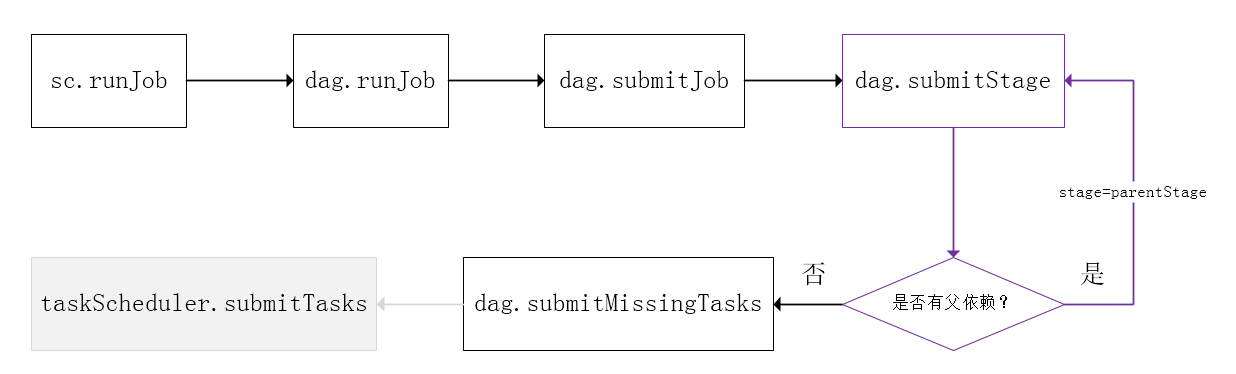
\includegraphics[width=0.99\textwidth]{dag-scheduler-process}
    \caption{DAG调度处理流程}
    \label{fig:dag-scheduler-process}
\end{figure}

Task级别调度是由TaskScheduler完成的。DAGScheduler会将Stage打包成TaskSet发送给TaskScheduler。TaskScheduler会为每一个TaskSet创建一个TaskSetManager来管理TaskSet。TaskScheduler会将新的TaskSetManager加入到队列等待调度执行。TaskScheduler启动之后会启动SchedulerBackend,SchedulerBackend是负责和外界沟通的。ResourceManager申请到资源后会启动Executor。SchedulerBackend负责和Executor通信。包括接受Executor的注册信息,记录Executor的状态。SchedulerBackend管理Executor也就相当于管理这物理资源,SchedulerBackend启动之后会定时询问TaskScheduler有没有任务调度需求。具体来说SchedulerBackend会给SchedulerBackend上报Executor剩余的资源,TaskScheduler会根据资源总量同时根据配置的调度策略调度一定数量的Task执行。

\begin{figure}
    \centering
    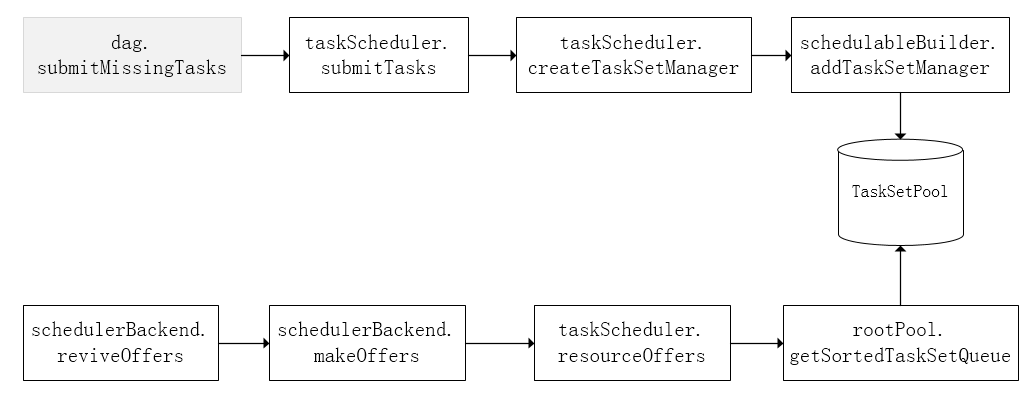
\includegraphics[width=0.99\textwidth]{task-scheduler-process}
    \caption{Task调度处理流程}
    \label{fig:task-scheduler-process}
\end{figure}

TaskSet被封装成TaskSetManager,TaskScheduler通过树形结构管理TaskSetManager。树的根节点类型为Schedule,叶子节点为TaskSetManager,中间非叶节点为Pool。TaskScheduler有两种调度策略,FIFO策略和FAIR策略。使用FIFO策略时TaskSetManager是以先来先出的方式进入队列。结构大概如\ref{fig:scheduler-fifo-tree}所示。

\begin{figure}
    \centering
    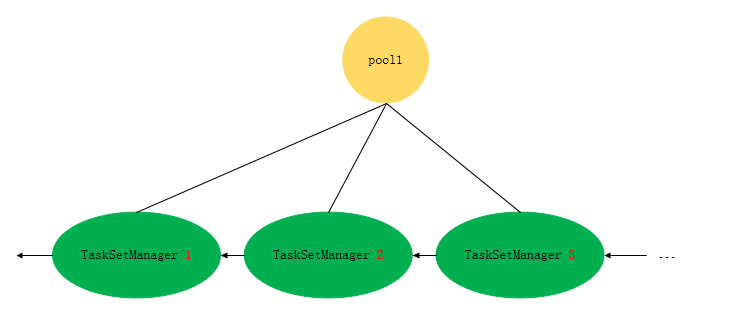
\includegraphics[width=0.99\textwidth]{Img/spark-scheduler-fifo-tree.png}
    \caption{FIFO调度策略底层树结构}
    \label{fig:scheduler-fifo-tree}
\end{figure}

FAIR调度策略用于保证多个作业的公平调度。比如有两个job,每个job的pool是不同的。FAIR调度会从根开始递归排序,首先对count-pool和take-pool排序。然后再对两个pool内部的TaskSetManager排序。排序的原则会考虑三个属性:runningTasks、minShare、Weight。通过三个属性进行比较的过程比较繁琐,最后能够保证的结果是不让资源被某些task长期占用,从而保证各个作业都能有调度执行的机会。

\begin{figure}
    \centering
    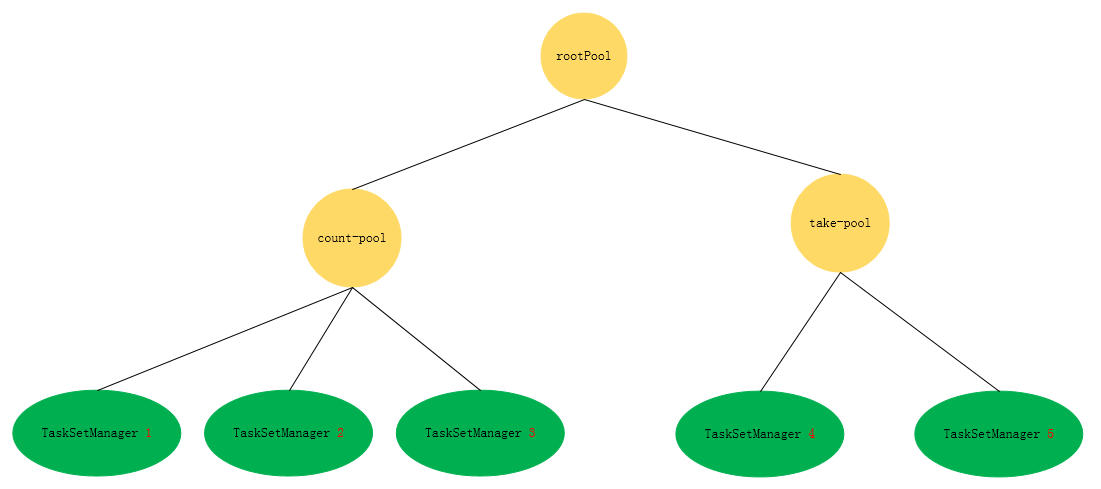
\includegraphics[width=0.99\textwidth]{Img/scheduler-fair-tree.png}
    \caption{FAIR调度策略底层树结构}
    \label{fig:scheduler-fair-tree}
\end{figure}

\subsection{缓存数据管理模块}

缓存存储模块主要包含如下两个部分,RDD缓存和Shuffle数据缓存。缓存模块的主要工作是管理RDD缓存,包括内存和磁盘的缓存。Shuffle中间数据的管理也是有缓存管理模块完成。存储模块中管理着多种不同的数据,包括RDD数据块、Shuffle数据块、广播变量数据块、任务返回数据块、流式数据块。RDD数据块用于标记缓存的RDD数据。Shuffle数据块用于标识缓存的Shuffle数据。广播变量数据块用于标识广播变量。任务返回数据块用于标识任务赶回结果数据。流式数据块在Spark Streaming中用于标记收到的流式数据。

RDD数据在缓存之前一般拥有多个

\section{缓存管理模块分析}
\subsection{Shuffle缓存}
\subsection{Storage缓存}
\subsection{Unroll缓存}
\section{本章总结}




